\PassOptionsToPackage{unicode=true}{hyperref} % options for packages loaded elsewhere
\PassOptionsToPackage{hyphens}{url}
%
\documentclass[]{article}
\usepackage{lmodern}
\usepackage{amssymb,amsmath}
\usepackage{ifxetex,ifluatex}
\usepackage{fixltx2e} % provides \textsubscript
\ifnum 0\ifxetex 1\fi\ifluatex 1\fi=0 % if pdftex
  \usepackage[T1]{fontenc}
  \usepackage[utf8]{inputenc}
  \usepackage{textcomp} % provides euro and other symbols
\else % if luatex or xelatex
  \usepackage{unicode-math}
  \defaultfontfeatures{Ligatures=TeX,Scale=MatchLowercase}
\fi
% use upquote if available, for straight quotes in verbatim environments
\IfFileExists{upquote.sty}{\usepackage{upquote}}{}
% use microtype if available
\IfFileExists{microtype.sty}{%
\usepackage[]{microtype}
\UseMicrotypeSet[protrusion]{basicmath} % disable protrusion for tt fonts
}{}
\IfFileExists{parskip.sty}{%
\usepackage{parskip}
}{% else
\setlength{\parindent}{0pt}
\setlength{\parskip}{6pt plus 2pt minus 1pt}
}
\usepackage{hyperref}
\hypersetup{
            pdftitle={Capstone Project},
            pdfborder={0 0 0},
            breaklinks=true}
\urlstyle{same}  % don't use monospace font for urls
\usepackage[margin=1in]{geometry}
\usepackage{color}
\usepackage{fancyvrb}
\newcommand{\VerbBar}{|}
\newcommand{\VERB}{\Verb[commandchars=\\\{\}]}
\DefineVerbatimEnvironment{Highlighting}{Verbatim}{commandchars=\\\{\}}
% Add ',fontsize=\small' for more characters per line
\usepackage{framed}
\definecolor{shadecolor}{RGB}{248,248,248}
\newenvironment{Shaded}{\begin{snugshade}}{\end{snugshade}}
\newcommand{\AlertTok}[1]{\textcolor[rgb]{0.94,0.16,0.16}{#1}}
\newcommand{\AnnotationTok}[1]{\textcolor[rgb]{0.56,0.35,0.01}{\textbf{\textit{#1}}}}
\newcommand{\AttributeTok}[1]{\textcolor[rgb]{0.77,0.63,0.00}{#1}}
\newcommand{\BaseNTok}[1]{\textcolor[rgb]{0.00,0.00,0.81}{#1}}
\newcommand{\BuiltInTok}[1]{#1}
\newcommand{\CharTok}[1]{\textcolor[rgb]{0.31,0.60,0.02}{#1}}
\newcommand{\CommentTok}[1]{\textcolor[rgb]{0.56,0.35,0.01}{\textit{#1}}}
\newcommand{\CommentVarTok}[1]{\textcolor[rgb]{0.56,0.35,0.01}{\textbf{\textit{#1}}}}
\newcommand{\ConstantTok}[1]{\textcolor[rgb]{0.00,0.00,0.00}{#1}}
\newcommand{\ControlFlowTok}[1]{\textcolor[rgb]{0.13,0.29,0.53}{\textbf{#1}}}
\newcommand{\DataTypeTok}[1]{\textcolor[rgb]{0.13,0.29,0.53}{#1}}
\newcommand{\DecValTok}[1]{\textcolor[rgb]{0.00,0.00,0.81}{#1}}
\newcommand{\DocumentationTok}[1]{\textcolor[rgb]{0.56,0.35,0.01}{\textbf{\textit{#1}}}}
\newcommand{\ErrorTok}[1]{\textcolor[rgb]{0.64,0.00,0.00}{\textbf{#1}}}
\newcommand{\ExtensionTok}[1]{#1}
\newcommand{\FloatTok}[1]{\textcolor[rgb]{0.00,0.00,0.81}{#1}}
\newcommand{\FunctionTok}[1]{\textcolor[rgb]{0.00,0.00,0.00}{#1}}
\newcommand{\ImportTok}[1]{#1}
\newcommand{\InformationTok}[1]{\textcolor[rgb]{0.56,0.35,0.01}{\textbf{\textit{#1}}}}
\newcommand{\KeywordTok}[1]{\textcolor[rgb]{0.13,0.29,0.53}{\textbf{#1}}}
\newcommand{\NormalTok}[1]{#1}
\newcommand{\OperatorTok}[1]{\textcolor[rgb]{0.81,0.36,0.00}{\textbf{#1}}}
\newcommand{\OtherTok}[1]{\textcolor[rgb]{0.56,0.35,0.01}{#1}}
\newcommand{\PreprocessorTok}[1]{\textcolor[rgb]{0.56,0.35,0.01}{\textit{#1}}}
\newcommand{\RegionMarkerTok}[1]{#1}
\newcommand{\SpecialCharTok}[1]{\textcolor[rgb]{0.00,0.00,0.00}{#1}}
\newcommand{\SpecialStringTok}[1]{\textcolor[rgb]{0.31,0.60,0.02}{#1}}
\newcommand{\StringTok}[1]{\textcolor[rgb]{0.31,0.60,0.02}{#1}}
\newcommand{\VariableTok}[1]{\textcolor[rgb]{0.00,0.00,0.00}{#1}}
\newcommand{\VerbatimStringTok}[1]{\textcolor[rgb]{0.31,0.60,0.02}{#1}}
\newcommand{\WarningTok}[1]{\textcolor[rgb]{0.56,0.35,0.01}{\textbf{\textit{#1}}}}
\usepackage{graphicx,grffile}
\makeatletter
\def\maxwidth{\ifdim\Gin@nat@width>\linewidth\linewidth\else\Gin@nat@width\fi}
\def\maxheight{\ifdim\Gin@nat@height>\textheight\textheight\else\Gin@nat@height\fi}
\makeatother
% Scale images if necessary, so that they will not overflow the page
% margins by default, and it is still possible to overwrite the defaults
% using explicit options in \includegraphics[width, height, ...]{}
\setkeys{Gin}{width=\maxwidth,height=\maxheight,keepaspectratio}
\setlength{\emergencystretch}{3em}  % prevent overfull lines
\providecommand{\tightlist}{%
  \setlength{\itemsep}{0pt}\setlength{\parskip}{0pt}}
\setcounter{secnumdepth}{0}
% Redefines (sub)paragraphs to behave more like sections
\ifx\paragraph\undefined\else
\let\oldparagraph\paragraph
\renewcommand{\paragraph}[1]{\oldparagraph{#1}\mbox{}}
\fi
\ifx\subparagraph\undefined\else
\let\oldsubparagraph\subparagraph
\renewcommand{\subparagraph}[1]{\oldsubparagraph{#1}\mbox{}}
\fi

% set default figure placement to htbp
\makeatletter
\def\fps@figure{htbp}
\makeatother


\title{Capstone Project}
\author{}
\date{\vspace{-2.5em}}

\begin{document}
\maketitle

\href{https://www.kaggle.com/proselotis/financial-ipo-data}{Data Source}

\begin{Shaded}
\begin{Highlighting}[]
\NormalTok{IPO =}\StringTok{ }\KeywordTok{read.csv}\NormalTok{(}\StringTok{"IPODataFull.csv"}\NormalTok{)}
\end{Highlighting}
\end{Shaded}

\hypertarget{data-cleaning}{%
\subsection{Data Cleaning}\label{data-cleaning}}

\begin{Shaded}
\begin{Highlighting}[]
\CommentTok{# default date in month}
\NormalTok{defaultDay =}\StringTok{ "15"}
\CommentTok{# default date in year}
\NormalTok{defaultDate =}\StringTok{"06-30"}
\end{Highlighting}
\end{Shaded}

\begin{Shaded}
\begin{Highlighting}[]
\CommentTok{# drop na in YearFounded}
\NormalTok{IPO =}\StringTok{ }\NormalTok{IPO[}\OperatorTok{!}\KeywordTok{is.na}\NormalTok{(IPO}\OperatorTok{$}\NormalTok{YearFounded),]}
\CommentTok{# look at original datetime format}
\CommentTok{# IPO %>% select(c("ipoDate", "YearFounded", "exactDateFounded"))}
\end{Highlighting}
\end{Shaded}

\begin{Shaded}
\begin{Highlighting}[]
\CommentTok{# subset of the original data set without TVC or anything after Fiscal_year}
\NormalTok{IPO_sub <-}\StringTok{ }\KeywordTok{select}\NormalTok{ (IPO, DaysToIPO, YearsToIPO, LastSale, Sector, Industry, CEOTakeOver, CEOAge, CEOGender, PresidentAge, Revenue, netIncome, lastFiscalYearGrowth, employees)}
\end{Highlighting}
\end{Shaded}

\begin{Shaded}
\begin{Highlighting}[]
\KeywordTok{summary}\NormalTok{(IPO_sub)}
\end{Highlighting}
\end{Shaded}

\begin{verbatim}
##    DaysToIPO       YearsToIPO       LastSale                       Sector   
##  Min.   :    0   Min.   :  0.0   Min.   :   0.0471   Health Care      :518  
##  1st Qu.:  486   1st Qu.:  1.0   1st Qu.:   7.0500   Finance          :472  
##  Median : 2359   Median :  6.0   Median :  17.4700   Consumer Services:463  
##  Mean   : 5379   Mean   : 14.7   Mean   :  31.0797   Technology       :393  
##  3rd Qu.: 5191   3rd Qu.: 14.0   3rd Qu.:  35.9800   Energy           :157  
##  Max.   :68021   Max.   :186.0   Max.   :1441.5000   Capital Goods    :149  
##                                                      (Other)          :669  
##                                     Industry     CEOTakeOver       CEOAge     
##  Major Pharmaceuticals                  : 302   Min.   :1965   Min.   :24.00  
##  Major Banks                            : 145   1st Qu.:2011   1st Qu.:50.00  
##  Business Services                      : 127   Median :2015   Median :55.00  
##  Real Estate Investment Trusts          : 126   Mean   :2013   Mean   :54.73  
##                                         : 118   3rd Qu.:2017   3rd Qu.:59.25  
##  Computer Software: Prepackaged Software: 104   Max.   :2018   Max.   :84.00  
##  (Other)                                :1899   NA's   :480    NA's   :277    
##          CEOGender     PresidentAge      Revenue             netIncome         
##               : 107   Min.   :24.00   Min.   :-3.250e+06   Min.   :-3.118e+12  
##  andy         :  46   1st Qu.:49.00   1st Qu.: 1.018e+08   1st Qu.:-2.146e+07  
##  female       : 115   Median :54.00   Median : 4.095e+08   Median : 6.890e+06  
##  male         :2223   Mean   :53.55   Mean   : 8.596e+10   Mean   : 5.853e+09  
##  mostly_female:  30   3rd Qu.:58.00   3rd Qu.: 1.625e+09   3rd Qu.: 1.039e+08  
##  mostly_male  :  51   Max.   :84.00   Max.   : 5.579e+13   Max.   : 6.620e+12  
##  unknown      : 249   NA's   :609     NA's   :422          NA's   :162         
##  lastFiscalYearGrowth   employees     
##  Min.   :  0.000      Min.   :     0  
##  1st Qu.:  0.080      1st Qu.:   142  
##  Median :  0.170      Median :   680  
##  Mean   :  1.957      Mean   :  7872  
##  3rd Qu.:  0.340      3rd Qu.:  3860  
##  Max.   :825.960      Max.   :566000  
##  NA's   :1119         NA's   :432
\end{verbatim}

\hypertarget{exploratory-analysis}{%
\subsection{Exploratory Analysis}\label{exploratory-analysis}}

\begin{Shaded}
\begin{Highlighting}[]
\KeywordTok{ggplot}\NormalTok{(}\DataTypeTok{data=}\NormalTok{IPO_sub,}\KeywordTok{aes}\NormalTok{(}\DataTypeTok{x=}\NormalTok{LastSale,}\DataTypeTok{y=}\NormalTok{DaysToIPO))}\OperatorTok{+}\KeywordTok{geom_point}\NormalTok{()}\OperatorTok{+}\KeywordTok{geom_smooth}\NormalTok{()}\OperatorTok{+}\KeywordTok{xlim}\NormalTok{(}\DecValTok{0}\NormalTok{, }\FloatTok{35.9800}\NormalTok{)}\OperatorTok{+}\KeywordTok{ylim}\NormalTok{(}\DecValTok{0}\NormalTok{,}\DecValTok{40000}\NormalTok{)}
\end{Highlighting}
\end{Shaded}

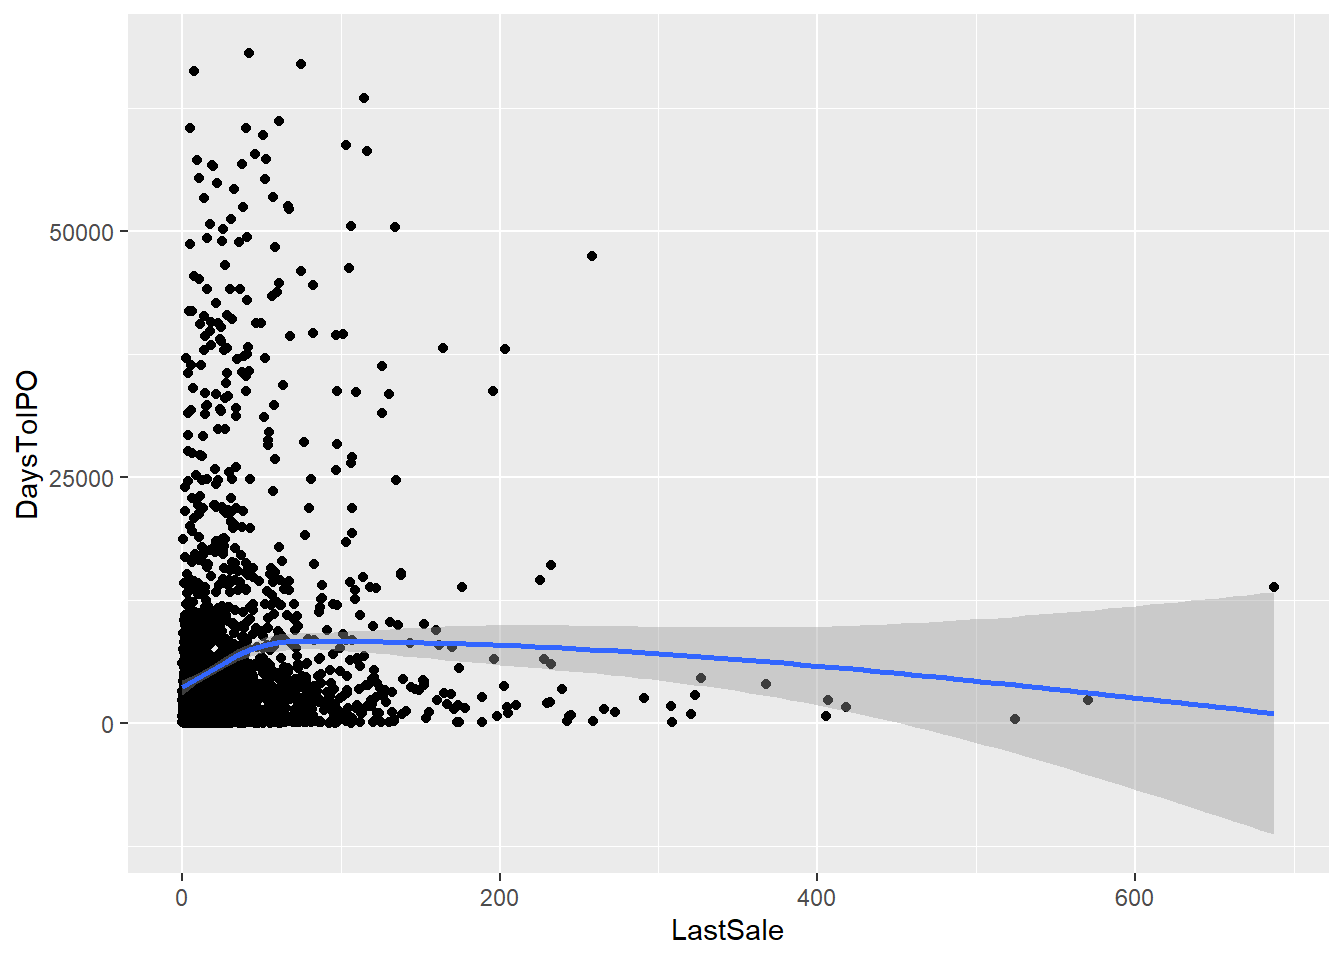
\includegraphics{Capstone-Project_files/figure-latex/unnamed-chunk-15-1.pdf}

\begin{Shaded}
\begin{Highlighting}[]
\KeywordTok{ggplot}\NormalTok{(}\DataTypeTok{data=}\NormalTok{IPO_sub,}\KeywordTok{aes}\NormalTok{(}\DataTypeTok{x=}\NormalTok{Revenue,}\DataTypeTok{y=}\NormalTok{DaysToIPO))}\OperatorTok{+}\KeywordTok{geom_point}\NormalTok{()}\OperatorTok{+}\KeywordTok{geom_smooth}\NormalTok{()}\OperatorTok{+}\KeywordTok{xlim}\NormalTok{(}\DecValTok{0}\NormalTok{, }\FloatTok{1.625e+09}\NormalTok{)}\OperatorTok{+}\KeywordTok{ylim}\NormalTok{(}\DecValTok{0}\NormalTok{,}\DecValTok{40000}\NormalTok{)}
\end{Highlighting}
\end{Shaded}

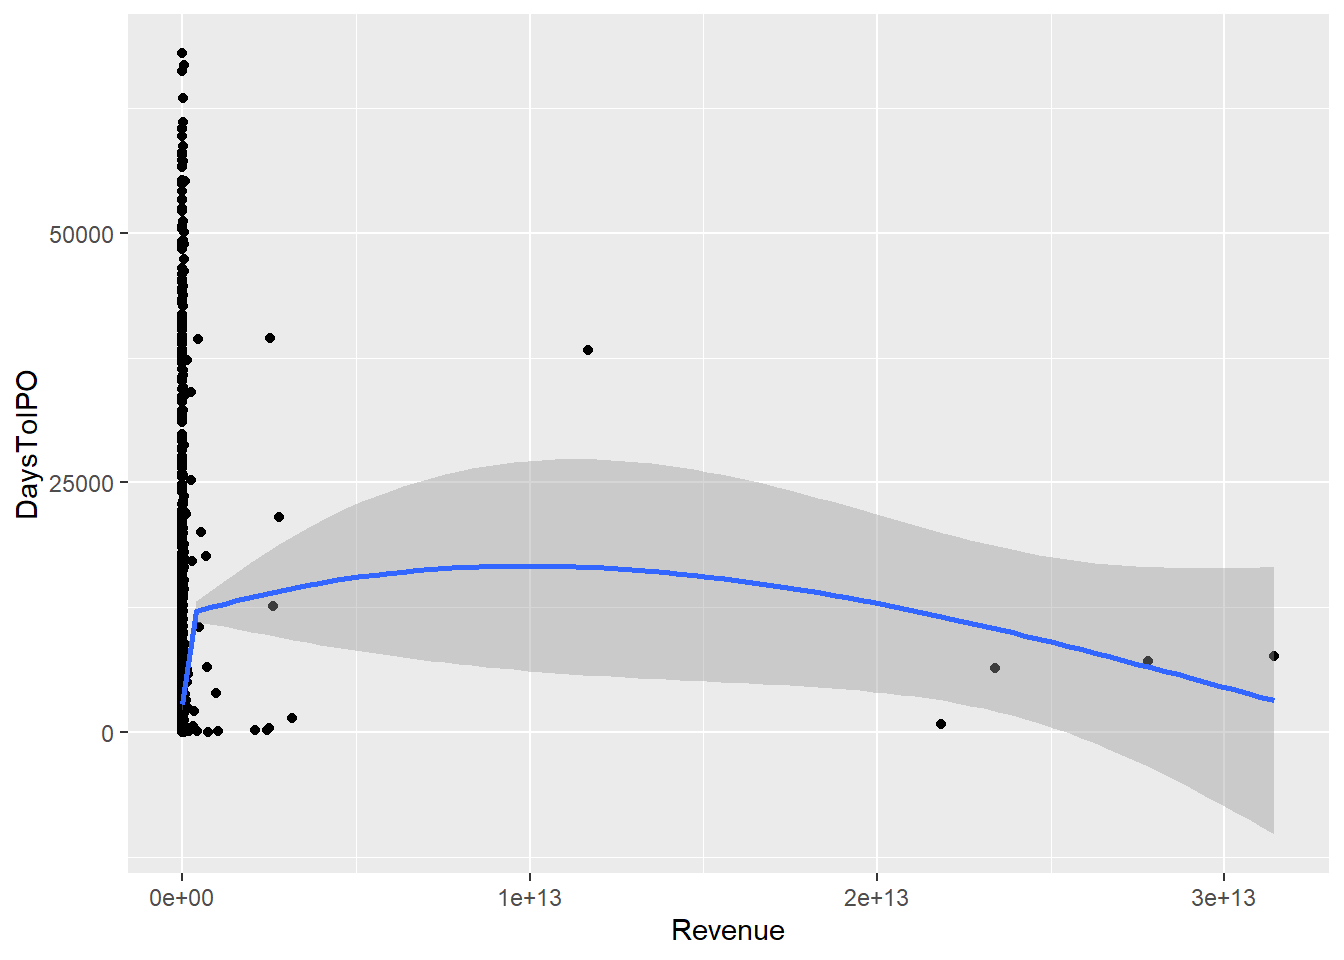
\includegraphics{Capstone-Project_files/figure-latex/unnamed-chunk-15-2.pdf}

\begin{Shaded}
\begin{Highlighting}[]
\KeywordTok{ggplot}\NormalTok{(}\DataTypeTok{data=}\NormalTok{IPO_sub,}\KeywordTok{aes}\NormalTok{(}\DataTypeTok{x=}\NormalTok{employees,}\DataTypeTok{y=}\NormalTok{DaysToIPO))}\OperatorTok{+}\KeywordTok{geom_point}\NormalTok{()}\OperatorTok{+}\KeywordTok{geom_smooth}\NormalTok{()}\OperatorTok{+}\KeywordTok{xlim}\NormalTok{(}\DecValTok{0}\NormalTok{, }\DecValTok{3860}\NormalTok{)}\OperatorTok{+}\KeywordTok{ylim}\NormalTok{(}\DecValTok{0}\NormalTok{,}\DecValTok{40000}\NormalTok{)}
\end{Highlighting}
\end{Shaded}

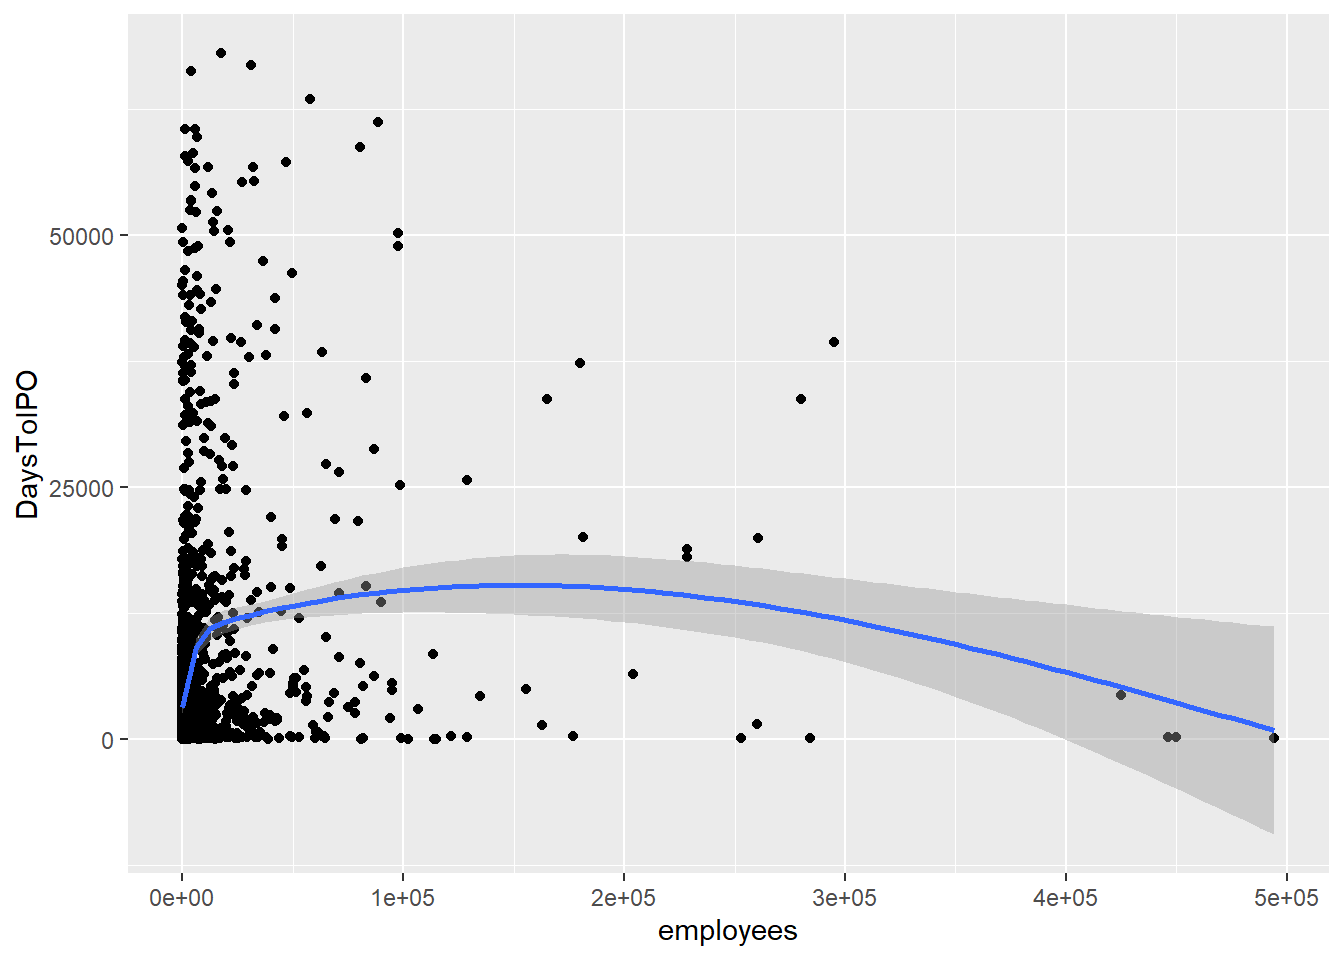
\includegraphics{Capstone-Project_files/figure-latex/unnamed-chunk-15-3.pdf}

\begin{Shaded}
\begin{Highlighting}[]
\KeywordTok{ggplot}\NormalTok{(}\DataTypeTok{data=}\NormalTok{IPO_sub2,}\KeywordTok{aes}\NormalTok{(}\DataTypeTok{x=}\NormalTok{LastSale,}\DataTypeTok{y=}\NormalTok{DaysToIPO))}\OperatorTok{+}\KeywordTok{geom_point}\NormalTok{()}\OperatorTok{+}\KeywordTok{geom_smooth}\NormalTok{()}
\end{Highlighting}
\end{Shaded}

\includegraphics{Capstone-Project_files/figure-latex/unnamed-chunk-17-1.pdf}

\begin{Shaded}
\begin{Highlighting}[]
\KeywordTok{ggplot}\NormalTok{(}\DataTypeTok{data=}\NormalTok{IPO_sub2,}\KeywordTok{aes}\NormalTok{(}\DataTypeTok{x=}\NormalTok{Revenue,}\DataTypeTok{y=}\NormalTok{DaysToIPO))}\OperatorTok{+}\KeywordTok{geom_point}\NormalTok{()}\OperatorTok{+}\KeywordTok{geom_smooth}\NormalTok{()}
\end{Highlighting}
\end{Shaded}

\includegraphics{Capstone-Project_files/figure-latex/unnamed-chunk-17-2.pdf}

\begin{Shaded}
\begin{Highlighting}[]
\KeywordTok{ggplot}\NormalTok{(}\DataTypeTok{data=}\NormalTok{IPO_sub2,}\KeywordTok{aes}\NormalTok{(}\DataTypeTok{x=}\NormalTok{employees,}\DataTypeTok{y=}\NormalTok{DaysToIPO))}\OperatorTok{+}\KeywordTok{geom_point}\NormalTok{()}\OperatorTok{+}\KeywordTok{geom_smooth}\NormalTok{()}
\end{Highlighting}
\end{Shaded}

\includegraphics{Capstone-Project_files/figure-latex/unnamed-chunk-17-3.pdf}

\begin{Shaded}
\begin{Highlighting}[]
\KeywordTok{ggplot}\NormalTok{(IPO_sub,}\KeywordTok{aes}\NormalTok{(}\DataTypeTok{x=}\NormalTok{Sector,}\DataTypeTok{y=}\NormalTok{DaysToIPO)) }\OperatorTok{+}
\StringTok{  }\KeywordTok{geom_boxplot}\NormalTok{() }\OperatorTok{+}\StringTok{ }
\StringTok{  }\KeywordTok{theme}\NormalTok{(}\DataTypeTok{axis.text.x =} \KeywordTok{element_text}\NormalTok{(}\DataTypeTok{angle =} \DecValTok{90}\NormalTok{))}
\end{Highlighting}
\end{Shaded}

\includegraphics{Capstone-Project_files/figure-latex/unnamed-chunk-18-1.pdf}

\hypertarget{modeling-with-daystoipo}{%
\subsection{Modeling with DaysToIPO}\label{modeling-with-daystoipo}}

\hypertarget{check-ph-assumption}{%
\subsubsection{Check PH assumption}\label{check-ph-assumption}}

\begin{Shaded}
\begin{Highlighting}[]
\NormalTok{m3 =}\StringTok{ }\KeywordTok{coxph}\NormalTok{( }\KeywordTok{Surv}\NormalTok{( DaysToIPO) }\OperatorTok{~}\StringTok{ }\NormalTok{Revenue , }\DataTypeTok{data=}\NormalTok{IPO_sub )}
\KeywordTok{plot}\NormalTok{( }\KeywordTok{cox.zph}\NormalTok{(m3) )}
\end{Highlighting}
\end{Shaded}

\includegraphics{Capstone-Project_files/figure-latex/unnamed-chunk-22-1.pdf}

\begin{Shaded}
\begin{Highlighting}[]
\NormalTok{m4 =}\StringTok{ }\KeywordTok{coxph}\NormalTok{( }\KeywordTok{Surv}\NormalTok{( DaysToIPO) }\OperatorTok{~}\StringTok{ }\NormalTok{netIncome , }\DataTypeTok{data=}\NormalTok{IPO_sub )}
\KeywordTok{plot}\NormalTok{( }\KeywordTok{cox.zph}\NormalTok{(m4) )}
\end{Highlighting}
\end{Shaded}

\includegraphics{Capstone-Project_files/figure-latex/unnamed-chunk-22-2.pdf}

\begin{Shaded}
\begin{Highlighting}[]
\NormalTok{m9 =}\StringTok{ }\KeywordTok{coxph}\NormalTok{( }\KeywordTok{Surv}\NormalTok{( DaysToIPO) }\OperatorTok{~}\StringTok{ }\NormalTok{LastSale , }\DataTypeTok{data=}\NormalTok{IPO_sub )}
\KeywordTok{plot}\NormalTok{( }\KeywordTok{cox.zph}\NormalTok{(m9) )}
\end{Highlighting}
\end{Shaded}

\includegraphics{Capstone-Project_files/figure-latex/unnamed-chunk-22-3.pdf}

\begin{Shaded}
\begin{Highlighting}[]
\CommentTok{# only m3, m4, m9 (Revenue, netIncome, LastSale satisfy the PH assumption)}

\KeywordTok{cox.zph}\NormalTok{(m3) }\CommentTok{## >  0.05}
\end{Highlighting}
\end{Shaded}

\begin{verbatim}
##         chisq df     p
## Revenue  2.99  1 0.084
## GLOBAL   2.99  1 0.084
\end{verbatim}

\begin{Shaded}
\begin{Highlighting}[]
\KeywordTok{cox.zph}\NormalTok{(m4) }\CommentTok{## >  0.05}
\end{Highlighting}
\end{Shaded}

\begin{verbatim}
##           chisq df    p
## netIncome 0.741  1 0.39
## GLOBAL    0.741  1 0.39
\end{verbatim}

\begin{Shaded}
\begin{Highlighting}[]
\KeywordTok{cox.zph}\NormalTok{(m9) }\CommentTok{## >  0.05}
\end{Highlighting}
\end{Shaded}

\begin{verbatim}
##           chisq df    p
## LastSale 0.0365  1 0.85
## GLOBAL   0.0365  1 0.85
\end{verbatim}

\begin{Shaded}
\begin{Highlighting}[]
\KeywordTok{coxph}\NormalTok{(}\KeywordTok{Surv}\NormalTok{(DaysToIPO)}\OperatorTok{~}\NormalTok{LastSale}\OperatorTok{+}\NormalTok{employees}\OperatorTok{+}\KeywordTok{strata}\NormalTok{(Industry)}\OperatorTok{+}\KeywordTok{strata}\NormalTok{(Sector)}\OperatorTok{+}\KeywordTok{strata}\NormalTok{(CEOGender)}\OperatorTok{+}\NormalTok{CEOAge}\OperatorTok{+}\NormalTok{PresidentAge}\OperatorTok{+}\NormalTok{Revenue}\OperatorTok{+}\NormalTok{netIncome}\OperatorTok{+}\NormalTok{lastFiscalYearGrowth,}\DataTypeTok{data=}\NormalTok{IPO_sub)}
\end{Highlighting}
\end{Shaded}

\begin{verbatim}
## Call:
## coxph(formula = Surv(DaysToIPO) ~ LastSale + employees + strata(Industry) + 
##     strata(Sector) + strata(CEOGender) + CEOAge + PresidentAge + 
##     Revenue + netIncome + lastFiscalYearGrowth, data = IPO_sub)
## 
##                            coef  exp(coef)   se(coef)      z      p
## LastSale             -7.637e-05  9.999e-01  7.910e-04 -0.097 0.9231
## employees            -4.886e-06  1.000e+00  2.447e-06 -1.996 0.0459
## CEOAge               -1.416e-02  9.859e-01  6.071e-03 -2.332 0.0197
## PresidentAge         -5.151e-03  9.949e-01  6.155e-03 -0.837 0.4027
## Revenue              -3.197e-12  1.000e+00  2.904e-12 -1.101 0.2709
## netIncome             1.913e-11  1.000e+00  1.544e-11  1.239 0.2153
## lastFiscalYearGrowth  1.081e-03  1.001e+00  8.241e-04  1.312 0.1894
## 
## Likelihood ratio test=24.13  on 7 df, p=0.00108
## n= 1280, number of events= 1280 
##    (1541 observations deleted due to missingness)
\end{verbatim}

\begin{Shaded}
\begin{Highlighting}[]
\KeywordTok{coxph}\NormalTok{(}\KeywordTok{Surv}\NormalTok{(DaysToIPO)}\OperatorTok{~}\NormalTok{CEOAge,}\DataTypeTok{data=}\NormalTok{IPO_sub) }\CommentTok{# significant}
\end{Highlighting}
\end{Shaded}

\begin{verbatim}
## Call:
## coxph(formula = Surv(DaysToIPO) ~ CEOAge, data = IPO_sub)
## 
##             coef exp(coef)  se(coef)      z        p
## CEOAge -0.013204  0.986883  0.002639 -5.003 5.65e-07
## 
## Likelihood ratio test=25.08  on 1 df, p=5.51e-07
## n= 2544, number of events= 2544 
##    (277 observations deleted due to missingness)
\end{verbatim}

\begin{Shaded}
\begin{Highlighting}[]
\KeywordTok{coxph}\NormalTok{(}\KeywordTok{Surv}\NormalTok{(DaysToIPO)}\OperatorTok{~}\NormalTok{PresidentAge,}\DataTypeTok{data=}\NormalTok{IPO_sub) }\CommentTok{# significant}
\end{Highlighting}
\end{Shaded}

\begin{verbatim}
## Call:
## coxph(formula = Surv(DaysToIPO) ~ PresidentAge, data = IPO_sub)
## 
##                   coef exp(coef)  se(coef)      z      p
## PresidentAge -0.006378  0.993642  0.002931 -2.176 0.0296
## 
## Likelihood ratio test=4.74  on 1 df, p=0.02949
## n= 2212, number of events= 2212 
##    (609 observations deleted due to missingness)
\end{verbatim}

\begin{Shaded}
\begin{Highlighting}[]
\KeywordTok{coxph}\NormalTok{(}\KeywordTok{Surv}\NormalTok{(DaysToIPO)}\OperatorTok{~}\NormalTok{LastSale,}\DataTypeTok{data=}\NormalTok{IPO_sub) }\CommentTok{# significant}
\end{Highlighting}
\end{Shaded}

\begin{verbatim}
## Call:
## coxph(formula = Surv(DaysToIPO) ~ LastSale, data = IPO_sub)
## 
##                coef  exp(coef)   se(coef)      z        p
## LastSale -0.0026896  0.9973141  0.0005146 -5.226 1.73e-07
## 
## Likelihood ratio test=32.15  on 1 df, p=1.426e-08
## n= 2821, number of events= 2821
\end{verbatim}

\begin{Shaded}
\begin{Highlighting}[]
\NormalTok{mod1=}\KeywordTok{survreg}\NormalTok{(}\KeywordTok{Surv}\NormalTok{(DaysToIPO}\FloatTok{+0.0001}\NormalTok{)}\OperatorTok{~}\NormalTok{LastSale}\OperatorTok{+}\NormalTok{employees}\OperatorTok{+}\NormalTok{CEOAge,}\DataTypeTok{data=}\NormalTok{IPO_sub,}\DataTypeTok{dist=}\StringTok{"weibull"}\NormalTok{)}
\KeywordTok{summary}\NormalTok{(mod1)}
\end{Highlighting}
\end{Shaded}

\begin{verbatim}
## 
## Call:
## survreg(formula = Surv(DaysToIPO + 1e-04) ~ LastSale + employees + 
##     CEOAge, data = IPO_sub, dist = "weibull")
##                Value Std. Error     z       p
## (Intercept) 7.19e+00   2.36e-01 30.40 < 2e-16
## LastSale    2.47e-03   7.89e-04  3.13  0.0018
## employees   1.03e-05   1.79e-06  5.76 8.6e-09
## CEOAge      1.76e-02   4.28e-03  4.12 3.8e-05
## Log(scale)  3.87e-01   1.63e-02 23.76 < 2e-16
## 
## Scale= 1.47 
## 
## Weibull distribution
## Loglik(model)= -20791.6   Loglik(intercept only)= -20838.2
##  Chisq= 93.35 on 3 degrees of freedom, p= 4.2e-20 
## Number of Newton-Raphson Iterations: 5 
## n=2203 (618 observations deleted due to missingness)
\end{verbatim}

\begin{Shaded}
\begin{Highlighting}[]
\NormalTok{mod2 =}\StringTok{ }\KeywordTok{survreg}\NormalTok{(}\KeywordTok{Surv}\NormalTok{(DaysToIPO}\FloatTok{+0.0001}\NormalTok{)}\OperatorTok{~}\NormalTok{LastSale}\OperatorTok{+}\NormalTok{employees}\OperatorTok{+}\NormalTok{CEOAge}\OperatorTok{+}\KeywordTok{factor}\NormalTok{(Sector),}\DataTypeTok{data=}\NormalTok{IPO_sub,}\DataTypeTok{dist=}\StringTok{"weibull"}\NormalTok{)}
\KeywordTok{summary}\NormalTok{(mod2)}
\end{Highlighting}
\end{Shaded}

\begin{verbatim}
## 
## Call:
## survreg(formula = Surv(DaysToIPO + 1e-04) ~ LastSale + employees + 
##     CEOAge + factor(Sector), data = IPO_sub, dist = "weibull")
##                                        Value Std. Error     z       p
## (Intercept)                         5.36e+00   2.96e-01 18.10 < 2e-16
## LastSale                            2.02e-03   7.65e-04  2.64  0.0083
## employees                           8.28e-06   1.68e-06  4.92 8.8e-07
## CEOAge                              1.98e-02   4.24e-03  4.67 3.0e-06
## factor(Sector)Basic Industries      1.83e+00   2.12e-01  8.63 < 2e-16
## factor(Sector)Capital Goods         2.17e+00   2.02e-01 10.72 < 2e-16
## factor(Sector)Consumer Durables     1.66e+00   2.61e-01  6.35 2.1e-10
## factor(Sector)Consumer Non-Durables 2.50e+00   2.27e-01 11.01 < 2e-16
## factor(Sector)Consumer Services     1.83e+00   1.74e-01 10.52 < 2e-16
## factor(Sector)Energy                1.76e+00   2.03e-01  8.68 < 2e-16
## factor(Sector)Finance               1.84e+00   1.73e-01 10.66 < 2e-16
## factor(Sector)Health Care           1.51e+00   1.71e-01  8.81 < 2e-16
## factor(Sector)Miscellaneous         1.91e+00   2.23e-01  8.58 < 2e-16
## factor(Sector)Public Utilities      2.21e+00   2.32e-01  9.49 < 2e-16
## factor(Sector)Technology            1.59e+00   1.78e-01  8.94 < 2e-16
## factor(Sector)Transportation        1.91e+00   2.62e-01  7.29 3.1e-13
## Log(scale)                          3.52e-01   1.64e-02 21.51 < 2e-16
## 
## Scale= 1.42 
## 
## Weibull distribution
## Loglik(model)= -20718.1   Loglik(intercept only)= -20838.2
##  Chisq= 240.31 on 15 degrees of freedom, p= 1.2e-42 
## Number of Newton-Raphson Iterations: 6 
## n=2203 (618 observations deleted due to missingness)
\end{verbatim}

\begin{Shaded}
\begin{Highlighting}[]
\KeywordTok{summary}\NormalTok{(}\KeywordTok{survreg}\NormalTok{(}\KeywordTok{Surv}\NormalTok{(DaysToIPO)}\OperatorTok{~}\NormalTok{LastSale}\OperatorTok{+}\NormalTok{employees}\OperatorTok{+}\NormalTok{CEOAge}\OperatorTok{+}\KeywordTok{factor}\NormalTok{(Sector),}\DataTypeTok{data=}\NormalTok{IPO_sub,}\DataTypeTok{dist=}\StringTok{"gaussian"}\NormalTok{)) }\CommentTok{# LastSale not significant}
\end{Highlighting}
\end{Shaded}

\begin{verbatim}
## 
## Call:
## survreg(formula = Surv(DaysToIPO) ~ LastSale + employees + CEOAge + 
##     factor(Sector), data = IPO_sub, dist = "gaussian")
##                                         Value Std. Error      z       p
## (Intercept)                         -4.09e+03   1.72e+03  -2.38 0.01739
## LastSale                             3.91e+00   3.85e+00   1.02 0.30948
## employees                            4.39e-02   7.64e-03   5.75 9.0e-09
## CEOAge                               9.52e+01   2.67e+01   3.56 0.00037
## factor(Sector)Basic Industries       5.02e+03   1.26e+03   3.98 6.9e-05
## factor(Sector)Capital Goods          6.94e+03   1.18e+03   5.89 3.9e-09
## factor(Sector)Consumer Durables      3.59e+03   1.62e+03   2.22 0.02629
## factor(Sector)Consumer Non-Durables  1.10e+04   1.36e+03   8.08 6.7e-16
## factor(Sector)Consumer Services      4.18e+03   9.63e+02   4.34 1.4e-05
## factor(Sector)Energy                 4.49e+03   1.19e+03   3.76 0.00017
## factor(Sector)Finance                4.98e+03   9.62e+02   5.18 2.3e-07
## factor(Sector)Health Care            2.22e+03   9.40e+02   2.37 0.01799
## factor(Sector)Miscellaneous          4.62e+03   1.34e+03   3.46 0.00055
## factor(Sector)Public Utilities       7.32e+03   1.41e+03   5.20 2.0e-07
## factor(Sector)Technology             2.46e+03   9.90e+02   2.49 0.01281
## factor(Sector)Transportation         5.85e+03   0.00e+00    Inf < 2e-16
## Log(scale)                           9.15e+00   1.51e-02 607.35 < 2e-16
## 
## Scale= 9413 
## 
## Gaussian distribution
## Loglik(model)= -23283.1   Loglik(intercept only)= -23371.7
##  Chisq= 177.06 on 15 degrees of freedom, p= 9.3e-30 
## Number of Newton-Raphson Iterations: 3 
## n=2203 (618 observations deleted due to missingness)
\end{verbatim}

\includegraphics{Capstone-Project_files/figure-latex/unnamed-chunk-37-1.pdf}

\begin{Shaded}
\begin{Highlighting}[]
\KeywordTok{summary}\NormalTok{(}\KeywordTok{survreg}\NormalTok{(}\KeywordTok{Surv}\NormalTok{(DaysToIPO}\FloatTok{+0.0001}\NormalTok{)}\OperatorTok{~}\NormalTok{LastSale}\OperatorTok{+}\NormalTok{employees}\OperatorTok{+}\NormalTok{CEOAge}\OperatorTok{+}\KeywordTok{factor}\NormalTok{(Sector),}\DataTypeTok{data=}\NormalTok{IPO_sub,}\DataTypeTok{dist=}\StringTok{"exponential"}\NormalTok{)) }\CommentTok{# significant}
\end{Highlighting}
\end{Shaded}

\begin{verbatim}
## 
## Call:
## survreg(formula = Surv(DaysToIPO + 1e-04) ~ LastSale + employees + 
##     CEOAge + factor(Sector), data = IPO_sub, dist = "exponential")
##                                        Value Std. Error     z       p
## (Intercept)                         5.93e+00   2.16e-01 27.49 < 2e-16
## LastSale                            2.17e-03   5.84e-04  3.73   2e-04
## employees                           9.53e-06   1.37e-06  6.94 4.0e-12
## CEOAge                              1.97e-02   3.09e-03  6.38 1.8e-10
## factor(Sector)Basic Industries      1.56e+00   1.49e-01 10.47 < 2e-16
## factor(Sector)Capital Goods         1.80e+00   1.42e-01 12.70 < 2e-16
## factor(Sector)Consumer Durables     1.34e+00   1.84e-01  7.31 2.6e-13
## factor(Sector)Consumer Non-Durables 2.15e+00   1.60e-01 13.45 < 2e-16
## factor(Sector)Consumer Services     1.51e+00   1.22e-01 12.33 < 2e-16
## factor(Sector)Energy                1.54e+00   1.43e-01 10.73 < 2e-16
## factor(Sector)Finance               1.55e+00   1.22e-01 12.77 < 2e-16
## factor(Sector)Health Care           1.06e+00   1.20e-01  8.82 < 2e-16
## factor(Sector)Miscellaneous         1.54e+00   1.57e-01  9.80 < 2e-16
## factor(Sector)Public Utilities      1.94e+00   1.64e-01 11.85 < 2e-16
## factor(Sector)Technology            1.13e+00   1.25e-01  9.01 < 2e-16
## factor(Sector)Transportation        1.61e+00   1.84e-01  8.75 < 2e-16
## 
## Scale fixed at 1 
## 
## Exponential distribution
## Loglik(model)= -20997.2   Loglik(intercept only)= -21260.4
##  Chisq= 526.33 on 15 degrees of freedom, p= 1.5e-102 
## Number of Newton-Raphson Iterations: 6 
## n=2203 (618 observations deleted due to missingness)
\end{verbatim}

\includegraphics{Capstone-Project_files/figure-latex/unnamed-chunk-39-1.pdf}

\begin{Shaded}
\begin{Highlighting}[]
\KeywordTok{summary}\NormalTok{(}\KeywordTok{survreg}\NormalTok{(}\KeywordTok{Surv}\NormalTok{(DaysToIPO}\FloatTok{+0.0001}\NormalTok{)}\OperatorTok{~}\NormalTok{LastSale}\OperatorTok{+}\NormalTok{employees}\OperatorTok{+}\NormalTok{CEOAge}\OperatorTok{+}\KeywordTok{factor}\NormalTok{(Sector),}\DataTypeTok{data=}\NormalTok{IPO_sub,}\DataTypeTok{dist=}\StringTok{"weibull"}\NormalTok{)) }\CommentTok{# significant}
\end{Highlighting}
\end{Shaded}

\begin{verbatim}
## 
## Call:
## survreg(formula = Surv(DaysToIPO + 1e-04) ~ LastSale + employees + 
##     CEOAge + factor(Sector), data = IPO_sub, dist = "weibull")
##                                        Value Std. Error     z       p
## (Intercept)                         5.36e+00   2.96e-01 18.10 < 2e-16
## LastSale                            2.02e-03   7.65e-04  2.64  0.0083
## employees                           8.28e-06   1.68e-06  4.92 8.8e-07
## CEOAge                              1.98e-02   4.24e-03  4.67 3.0e-06
## factor(Sector)Basic Industries      1.83e+00   2.12e-01  8.63 < 2e-16
## factor(Sector)Capital Goods         2.17e+00   2.02e-01 10.72 < 2e-16
## factor(Sector)Consumer Durables     1.66e+00   2.61e-01  6.35 2.1e-10
## factor(Sector)Consumer Non-Durables 2.50e+00   2.27e-01 11.01 < 2e-16
## factor(Sector)Consumer Services     1.83e+00   1.74e-01 10.52 < 2e-16
## factor(Sector)Energy                1.76e+00   2.03e-01  8.68 < 2e-16
## factor(Sector)Finance               1.84e+00   1.73e-01 10.66 < 2e-16
## factor(Sector)Health Care           1.51e+00   1.71e-01  8.81 < 2e-16
## factor(Sector)Miscellaneous         1.91e+00   2.23e-01  8.58 < 2e-16
## factor(Sector)Public Utilities      2.21e+00   2.32e-01  9.49 < 2e-16
## factor(Sector)Technology            1.59e+00   1.78e-01  8.94 < 2e-16
## factor(Sector)Transportation        1.91e+00   2.62e-01  7.29 3.1e-13
## Log(scale)                          3.52e-01   1.64e-02 21.51 < 2e-16
## 
## Scale= 1.42 
## 
## Weibull distribution
## Loglik(model)= -20718.1   Loglik(intercept only)= -20838.2
##  Chisq= 240.31 on 15 degrees of freedom, p= 1.2e-42 
## Number of Newton-Raphson Iterations: 6 
## n=2203 (618 observations deleted due to missingness)
\end{verbatim}

\includegraphics{Capstone-Project_files/figure-latex/unnamed-chunk-41-1.pdf}

\begin{Shaded}
\begin{Highlighting}[]
\KeywordTok{summary}\NormalTok{(}\KeywordTok{survreg}\NormalTok{(}\KeywordTok{Surv}\NormalTok{(DaysToIPO}\FloatTok{+0.0001}\NormalTok{)}\OperatorTok{~}\NormalTok{LastSale}\OperatorTok{+}\NormalTok{employees}\OperatorTok{+}\NormalTok{CEOAge}\OperatorTok{+}\KeywordTok{factor}\NormalTok{(Sector),}\DataTypeTok{data=}\NormalTok{IPO_sub,}\DataTypeTok{dist=}\StringTok{"lognormal"}\NormalTok{)) }\CommentTok{# LastSale not significant}
\end{Highlighting}
\end{Shaded}

\begin{verbatim}
## 
## Call:
## survreg(formula = Surv(DaysToIPO + 1e-04) ~ LastSale + employees + 
##     CEOAge + factor(Sector), data = IPO_sub, dist = "lognormal")
##                                        Value Std. Error     z       p
## (Intercept)                         4.66e+00   3.50e-01 13.30 < 2e-16
## LastSale                            1.43e-03   7.37e-04  1.94   0.052
## employees                           3.06e-06   1.46e-06  2.09   0.037
## CEOAge                              1.30e-02   5.12e-03  2.55   0.011
## factor(Sector)Basic Industries      1.98e+00   2.68e-01  7.39 1.5e-13
## factor(Sector)Capital Goods         2.37e+00   2.54e-01  9.34 < 2e-16
## factor(Sector)Consumer Durables     1.86e+00   3.31e-01  5.62 1.9e-08
## factor(Sector)Consumer Non-Durables 2.78e+00   2.86e-01  9.71 < 2e-16
## factor(Sector)Consumer Services     2.03e+00   2.18e-01  9.28 < 2e-16
## factor(Sector)Energy                1.80e+00   2.57e-01  7.03 2.0e-12
## factor(Sector)Finance               1.85e+00   2.18e-01  8.49 < 2e-16
## factor(Sector)Health Care           2.23e+00   2.14e-01 10.42 < 2e-16
## factor(Sector)Miscellaneous         2.35e+00   2.81e-01  8.37 < 2e-16
## factor(Sector)Public Utilities      2.13e+00   2.94e-01  7.27 3.6e-13
## factor(Sector)Technology            2.30e+00   2.22e-01 10.35 < 2e-16
## factor(Sector)Transportation        2.12e+00   3.30e-01  6.43 1.3e-10
## Log(scale)                          5.89e-01   1.51e-02 39.12 < 2e-16
## 
## Scale= 1.8 
## 
## Log Normal distribution
## Loglik(model)= -20921.7   Loglik(intercept only)= -21002.3
##  Chisq= 161.31 on 15 degrees of freedom, p= 1.3e-26 
## Number of Newton-Raphson Iterations: 3 
## n=2203 (618 observations deleted due to missingness)
\end{verbatim}

\includegraphics{Capstone-Project_files/figure-latex/unnamed-chunk-43-1.pdf}

\hypertarget{model-comparison}{%
\subsubsection{Model comparison}\label{model-comparison}}

\hypertarget{is-including-sector-worthwhile-yes}{%
\paragraph{is including Sector worthwhile?
Yes}\label{is-including-sector-worthwhile-yes}}

\begin{Shaded}
\begin{Highlighting}[]
\NormalTok{l1=}\KeywordTok{summary}\NormalTok{(mod1)}\OperatorTok{$}\NormalTok{loglik[}\DecValTok{2}\NormalTok{]}
\NormalTok{l2=}\KeywordTok{summary}\NormalTok{(mod2)}\OperatorTok{$}\NormalTok{loglik[}\DecValTok{2}\NormalTok{]}
\DecValTok{1} \OperatorTok{-}\StringTok{ }\KeywordTok{pchisq}\NormalTok{(}\DecValTok{2}\OperatorTok{*}\NormalTok{(l2}\OperatorTok{-}\NormalTok{l1),}\DecValTok{12}\NormalTok{) }\CommentTok{# = 0}
\end{Highlighting}
\end{Shaded}

\begin{verbatim}
## [1] 0
\end{verbatim}

\hypertarget{weibull-vs-normal-weibull}{%
\paragraph{weibull vs normal
(weibull)}\label{weibull-vs-normal-weibull}}

agrees with CS plot

\begin{Shaded}
\begin{Highlighting}[]
\NormalTok{loglik_weibull =}\StringTok{ }\FloatTok{-20718.1}
\NormalTok{loglik_normal =}\StringTok{ }\FloatTok{-23283.1}
\NormalTok{loglik_exponential =}\StringTok{ }\FloatTok{-20997.2}
\NormalTok{loglik_lognormal =}\StringTok{ }\FloatTok{-20921.7} 

\CommentTok{# AIC - not nested }
\DecValTok{2}\OperatorTok{*}\NormalTok{(}\DecValTok{16}\OperatorTok{-}\NormalTok{(loglik_weibull))}
\end{Highlighting}
\end{Shaded}

\begin{verbatim}
## [1] 41468.2
\end{verbatim}

\begin{Shaded}
\begin{Highlighting}[]
\DecValTok{2}\OperatorTok{*}\NormalTok{(}\DecValTok{16}\OperatorTok{-}\NormalTok{(loglik_normal))}
\end{Highlighting}
\end{Shaded}

\begin{verbatim}
## [1] 46598.2
\end{verbatim}

\hypertarget{weibull-vs-exponential-weibull}{%
\paragraph{weibull vs exponential
(weibull)}\label{weibull-vs-exponential-weibull}}

agrees with CS plot

\begin{Shaded}
\begin{Highlighting}[]
\CommentTok{# LRT - nested}
\NormalTok{ts=}\DecValTok{2}\OperatorTok{*}\NormalTok{(loglik_weibull}\OperatorTok{-}\NormalTok{(loglik_exponential))}
\DecValTok{1}\OperatorTok{-}\KeywordTok{pchisq}\NormalTok{(ts,}\DecValTok{1}\NormalTok{)}
\end{Highlighting}
\end{Shaded}

\begin{verbatim}
## [1] 0
\end{verbatim}

\begin{Shaded}
\begin{Highlighting}[]
\CommentTok{# AIC}
\DecValTok{2}\OperatorTok{*}\NormalTok{(}\DecValTok{16}\OperatorTok{-}\NormalTok{(loglik_weibull))}
\end{Highlighting}
\end{Shaded}

\begin{verbatim}
## [1] 41468.2
\end{verbatim}

\begin{Shaded}
\begin{Highlighting}[]
\DecValTok{2}\OperatorTok{*}\NormalTok{(}\DecValTok{15}\OperatorTok{-}\NormalTok{(loglik_exponential))}
\end{Highlighting}
\end{Shaded}

\begin{verbatim}
## [1] 42024.4
\end{verbatim}

\hypertarget{weibull-vs-log-normal-weibull}{%
\paragraph{weibull vs log-normal
(weibull)}\label{weibull-vs-log-normal-weibull}}

agrees with CS plot

\begin{Shaded}
\begin{Highlighting}[]
\CommentTok{# AIC - not nested }
\DecValTok{2}\OperatorTok{*}\NormalTok{(}\DecValTok{16}\OperatorTok{-}\NormalTok{(loglik_weibull))}
\end{Highlighting}
\end{Shaded}

\begin{verbatim}
## [1] 41468.2
\end{verbatim}

\begin{Shaded}
\begin{Highlighting}[]
\DecValTok{2}\OperatorTok{*}\NormalTok{(}\DecValTok{16}\OperatorTok{-}\NormalTok{(loglik_lognormal))}
\end{Highlighting}
\end{Shaded}

\begin{verbatim}
## [1] 41875.4
\end{verbatim}

\hypertarget{normal-vs-exponential-exponential}{%
\paragraph{normal vs exponential
(exponential)}\label{normal-vs-exponential-exponential}}

\begin{Shaded}
\begin{Highlighting}[]
\CommentTok{# AIC - not nested}
\DecValTok{2}\OperatorTok{*}\NormalTok{(}\DecValTok{16}\OperatorTok{-}\NormalTok{(loglik_normal))}
\end{Highlighting}
\end{Shaded}

\begin{verbatim}
## [1] 46598.2
\end{verbatim}

\begin{Shaded}
\begin{Highlighting}[]
\DecValTok{2}\OperatorTok{*}\NormalTok{(}\DecValTok{16}\OperatorTok{-}\NormalTok{(loglik_exponential))}
\end{Highlighting}
\end{Shaded}

\begin{verbatim}
## [1] 42026.4
\end{verbatim}

\hypertarget{normal-vs-log-normal-log-normal}{%
\paragraph{normal vs log-normal
(log-normal)}\label{normal-vs-log-normal-log-normal}}

\begin{Shaded}
\begin{Highlighting}[]
\CommentTok{# AIC - not nested}
\DecValTok{2}\OperatorTok{*}\NormalTok{(}\DecValTok{16}\OperatorTok{-}\NormalTok{(loglik_normal))}
\end{Highlighting}
\end{Shaded}

\begin{verbatim}
## [1] 46598.2
\end{verbatim}

\begin{Shaded}
\begin{Highlighting}[]
\DecValTok{2}\OperatorTok{*}\NormalTok{(}\DecValTok{16}\OperatorTok{-}\NormalTok{(loglik_lognormal))}
\end{Highlighting}
\end{Shaded}

\begin{verbatim}
## [1] 41875.4
\end{verbatim}

\hypertarget{exponential-vs-log-normal-log-normal}{%
\paragraph{exponential vs log-normal
(log-normal)}\label{exponential-vs-log-normal-log-normal}}

\begin{Shaded}
\begin{Highlighting}[]
\CommentTok{# AIC - not nested }
\DecValTok{2}\OperatorTok{*}\NormalTok{(}\DecValTok{15}\OperatorTok{-}\NormalTok{(loglik_exponential))}
\end{Highlighting}
\end{Shaded}

\begin{verbatim}
## [1] 42024.4
\end{verbatim}

\begin{Shaded}
\begin{Highlighting}[]
\DecValTok{2}\OperatorTok{*}\NormalTok{(}\DecValTok{16}\OperatorTok{-}\NormalTok{(loglik_lognormal))}
\end{Highlighting}
\end{Shaded}

\begin{verbatim}
## [1] 41875.4
\end{verbatim}

\hypertarget{modeling-with-yearstoipo}{%
\subsection{Modeling with YearsToIPO}\label{modeling-with-yearstoipo}}

\hypertarget{some-models}{%
\subsubsection{Some models}\label{some-models}}

\hypertarget{model-comparison-1}{%
\subsubsection{Model comparison}\label{model-comparison-1}}

\hypertarget{weibull-vs-normal-weibull-1}{%
\paragraph{weibull vs normal
(weibull)}\label{weibull-vs-normal-weibull-1}}

\hypertarget{weibull-vs-exponential-weibull-1}{%
\paragraph{weibull vs exponential
(weibull)}\label{weibull-vs-exponential-weibull-1}}

\hypertarget{weibull-vs-log-normal-weibull-1}{%
\paragraph{weibull vs log-normal
(weibull)}\label{weibull-vs-log-normal-weibull-1}}

\hypertarget{normal-vs-exponential-exponential-1}{%
\paragraph{normal vs exponential
(exponential)}\label{normal-vs-exponential-exponential-1}}

\hypertarget{normal-vs-log-normal-log-normal-1}{%
\paragraph{normal vs log-normal
(log-normal)}\label{normal-vs-log-normal-log-normal-1}}

\hypertarget{exponential-vs-log-normal-log-normal-1}{%
\paragraph{exponential vs log-normal
(log-normal)}\label{exponential-vs-log-normal-log-normal-1}}

\end{document}
